\documentclass[11pt]{article}
\usepackage[utf8]{inputenc}    
\usepackage[T1]{fontenc}  
\usepackage{amsmath}   
\usepackage{bm}  
\usepackage{amssymb}
\usepackage{amsmath} 
\usepackage{forest}
\usepackage{tikz}

\title{AT3 - Métodos Matemáticos para Gestão da Informação}
\date{}
\author{Juliane Pires}
\begin{document}
\maketitle

% Questão 1
\subsubsection*{1. Uma plataforma de conteúdos educacionais observou que o engajamento médio dos usuários depende do número de notificações semanais enviadas. Um modelo simplificado para esse comportamento é dado por:}
\[ E(x) = -2x^2 + 16x + 10 \]
\subsubsection*{onde $x$ = número de notificações por semana e $E(x)$ = índice de engajamento}
\subsubsection*{Tarefas:}

\subsubsection*{Identifique o sinal do coeficiente $a$ e explique o que isso indica sobre o formato da curva.}
O sinal do coeficiente $a$ (-2) é negativo, ou seja, isso indica que a parábola estará voltada pra baixo. Neste problema, é procurado um $\underline{\text{ponto de máximo}}$.
\subsubsection*{b) Calcule o vértice da função.}
\paragraph{$X_v$:}
\[ x_v = \frac{-b}{2a} = \frac{-16}{2(-2)} = \frac{-16}{-4} = 4 \therefore x = 4\]

\paragraph{$Y_v$:}
\[ E(4) = -2(4)^2 + 16(4) + 10 \]
\[ E(4) = -2(16) + 64 + 10 \]
\[ E(4) = -32 + 64 + 10 = 42 \therefore y = 42\]
O vértice é $\mathbf{V(4, 42)}$

\subsubsection*{c) Interprete o significado do vértice no contexto do problema.}
No contexto do problema, o $X_v$ indica o ponto em que a quantidade de notificações por semana (4). Já o $Y_v$ indica o índice máximo de engajamento que a plataforma atinge com essa quantidade de notificações semanais.

\subsubsection*{d) Faça um esboço do gráfico.}
\begin{center}
\begin{tikzpicture}[xscale=0.6, yscale=0.12, >=stealth] 
    
    \draw[->] (-1,0) -- (10,0) node[right, font=\tiny] {$x$};
    \draw[->] (0,-2) -- (0,50) node[above, font=\tiny] {$E(x)$};
    
    \draw[domain=0:8.5, smooth, variable=\x, blue, thick] 
        plot ({\x},{-2*\x*\x + 16*\x + 10});
    
    \filldraw[red] (4,42) node[above right, font=\scriptsize] {$V(4, 42)$};
    \draw[dashed, gray, very thin] (4,0) -- (4,42) -- (0,42);
    
    \filldraw[black] (0,10) node[left, font=\tiny] {10};
    
\end{tikzpicture}
\end{center}

\subsubsection*{e) Responda: Qual é o número ideal de notificações semanais? O que acontece se a plataforma enviar notificações em excesso?}
O número ideal é de \textbf{4 notificações por semana} ($x = 4$). Caso a plataforma envie mais do que 4 notificações na semana, o engajamento começa a cair, podendo ficar menor do que o índice inicial de 10 ou chegar a zero devido ao incômodo aos usuários.

% Questão 2
\subsubsection*{2. Uma equipe de Gestão da Informação modelou o custo anual de manutenção de uma base de dados em função do número de atualizações realizadas por ano. O modelo obtido foi:}

\[ C(x) = x^2 - 12x + 50 \]
\subsubsection*{onde $x$ = número de atualizações por ano e $C(x)$ = custo total (em unidades monetárias)}

\subsubsection*{a) Identifique o sinal do coeficiente $a$ e explique o que isso indica sobre o formato da curva.}
O sinal do coeficiente $a$ é positivo, ou seja, a parábola estará voltada para cima. Aqui, procura-se um ponto de mínimo.

\subsubsection*{b) Calcule o vértice da função.}

\paragraph{$X_v$:}
\[ x_v = \frac{-b}{2a} = \frac{-(-12)}{2(1)} = \frac{12}{2} = 6 \]

\paragraph{$Y_v$:}
\[ C(6) = (6)^2 - 12(6) + 50 \]
\[ C(6) = 36 - 72 + 50 \]
\[ C(6) = -36 + 50 = 14 \]
O vértice é $\mathbf{V(6, 14)}$.

\subsubsection*{c) Interprete o significado do vértice no contexto do problema.}

O resultado mostra que o número ideal de atualizações por ano ($x$) é igual a 6. Já o $Y_v$ representa o custo mínimo anual, que é de 14 unidades monetárias.

\subsubsection*{d) Faça um esboço do gráfico.}

\begin{center}
\begin{tikzpicture}[xscale=0.5, yscale=0.1, >=stealth] 
    % xscale=0.5 (largura reduzida) | yscale=0.1 (altura bem achatada)
    
    % Eixos
    \draw[->] (-1,0) -- (13,0) node[right, font=\tiny] {$x$};
    \draw[->] (0,-5) -- (0,55) node[above, font=\tiny] {$C(x)$};
    
    % Curva: C(x) = x^2 - 12x + 50
    \draw[domain=0:12, smooth, variable=\x, red, thick] 
        plot ({\x},{\x*\x - 12*\x + 50});
    
    % Vértice V(6, 14) - Ponto de Mínimo
    \filldraw[blue] (6,14) node[below, font=\tiny, yshift=-2pt] {$V(6, 14)$};
    \draw[dashed, gray, very thin] (6,0) -- (6,14) -- (0,14);
    
    % Intercepto y=50 (Custo Inicial)
    \filldraw[black] (0,50) node[left, font=\tiny] {50};
\end{tikzpicture}
\end{center}

\subsubsection*{e) Responda: Quantas atualizações por ano minimizam o custo? Por que atualizar menos ou mais do que isso aumenta o custo total?}
É possível minimizar o custo com 6 atualizações por ano. Se houver menos de 6 atualizações, o custo pode aumentar devido à falta de manutenção consistente. Já se houver mais de 6 atualizações, o custo pode aumentar devido ao excesso de processamento e demanda operacional desnecessária.

% Questão 3
\subsubsection*{3. Uma equipe de Gestão da Informação está avaliando um pipeline de tratamento de dados. A qualidade média da informação aumenta com o tempo de processamento no início, mas depois começa a cair devido à introdução de ruídos e redundâncias. Esse comportamento é modelado por:}
\[ Q(x) = -x^2 + 12x + 5 \]
\subsubsection*{Ao mesmo tempo, o tempo de processamento acumulado cresce de forma linear:}
\[ T(x) = 3x + 5 \]

\subsubsection*{onde:\\
$x$ = número de horas de processamento\\
$Q(x)$ = índice de qualidade da informação\\
$T(x)$ = custo temporal do processamento
}

\subsubsection*{a) Monte o sistema de equações que representa o momento em que qualidade e tempo possuem o mesmo valor numérico.}
\[
\begin{cases}
    y = -x^2 + 12x + 5 \\
    y = 3x + 5
\end{cases}
\]

\subsubsection*{b) Resolva o sistema.}
\[ -x^2 + 12x + 5 = 3x + 5 \]
\[ -x^2 + 9x = 0 \]
\[ x(-x + 9) = 0 \]

\begin{itemize}
    \item $x_1 = 0$
    \item $x_2 = 9$
\end{itemize}

Substituindo em $T(x)$ para encontrar $y$:
\begin{itemize}
    \item Para $x = 0: y = 3(0) + 5 = 5 \therefore P_1(0, 5)$
    \item Para $x = 9: y = 3(9) + 5 = 32 \therefore P_2(9, 32)$
\end{itemize}

\subsubsection*{c) Interprete o significado da solução encontrada.}
No início do processamento ($x = 0$), ambas as variáveis de ganho de qualidade e custo temporal partem do valor 5. Após 9 horas de processamento, esses valores voltam a se equilibrar no índice 32.

\subsubsection*{d) Esboce o gráfico e identifique o ponto de intersecção.}

\begin{center}
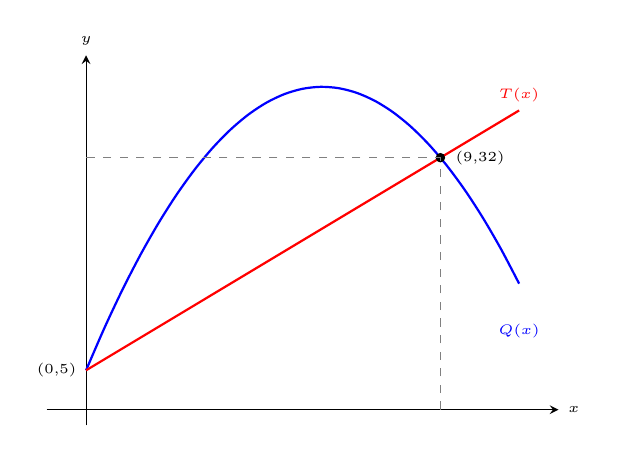
\begin{tikzpicture}[xscale=0.5, yscale=0.1, >=stealth]
    \draw[->] (-1,0) -- (12,0) node[right, font=\tiny] {$x$};
    \draw[->] (0,-2) -- (0,45) node[above, font=\tiny] {$y$};
    
    \draw[domain=0:11, smooth, variable=\x, blue, thick] plot ({\x}, {-\x*\x + 12*\x + 5});
    \node[blue, font=\tiny] at (11,10) {$Q(x)$};
    
    \draw[domain=0:11, smooth, variable=\x, red, thick] plot ({\x}, {3*\x + 5});
    \node[red, font=\tiny] at (11,40) {$T(x)$};
    
    \filldraw[black] (0,5) node[left, font=\tiny] {(0,5)};
    \filldraw[black] (9,32) circle (3pt and 15pt) node[right, font=\tiny, xshift=2pt] {(9,32)};    
    \draw[dashed, gray, very thin] (9,0) -- (9,32) -- (0,32);
\end{tikzpicture}
\end{center}

\subsubsection*{e) Em que intervalo o ganho de qualidade supera o custo de tempo?}

Quando $Q(x) > T(x)$, ou seja, no intervalo:
\[ \mathbf{0 < x < 9} \]

\subsubsection*{f) Explique o que esse resultado indica para a tomada de decisão do gestor.}

O resultado indica que gestor deve operar no intervalo em que o processamento é vantajoso, ou seja, até a 9ª hora. A pipeline deve ser interrompida antes desse limite, no ponto de máxima qualidade ($x=6$), pois o custo temporal e a perda de qualidade deixam a operação ineficiente após 9horas.


\subsubsection*{4. Uma empresa comercializa três tipos de serviços: Plano A, Plano B e Plano C.
Em três dias diferentes, foram registrados os seguintes faturamentos:\\
Dia 1: A + 2B + C → R\$ 21\\
Dia 2: 2A + B + 3C → R\$ 32\\
Dia 3: 3A + B + 2C → R\$ 37\\
Considere:\\
$x$ = valor do Plano A\\
$y$ = valor do Plano B\\
$z$ = valor do Plano C}

\subsubsection*{a) Monte o sistema linear.}
\[
\begin{cases}
    x + 2y + z = 21 \\
    2x + y + 3z = 32 \\
    3x + y + 2z = 37
\end{cases}
\]

\subsubsection*{b) Resolva por Gauss.}
Matriz aumentada:
\[
\left[
\begin{array}{ccc|c}
    1 & 2 & 1 & 21 \\
    2 & 1 & 3 & 32 \\
    3 & 1 & 2 & 37
\end{array}
\right]
\]

\paragraph{1:} Zerar a segunda linha, primeira coluna e a terceira linha, primeira coluna:
$L_2 \leftarrow L_2 - 2L_1$ e $L_3 \leftarrow L_3 - 3L_1$:
\[
\left[
\begin{array}{ccc|c}
    1 & 2 & 1 & 21 \\
    0 & -3 & 1 & -10 \\
    0 & -5 & -1 & -26
\end{array}
\right]
\]

\paragraph{2:} Zerar a terceira linha, segunda coluna:
$L_3 \leftarrow L_3 - \frac{5}{3}L_2$:
\[
\left[
\begin{array}{ccc|c}
    1 & 2 & 1 & 21 \\
    0 & -3 & 1 & -10 \\
    0 & 0 & -8/3 & -28/3
\end{array}
\right]
\]

\paragraph{Substituindo:}
\begin{itemize}
    \item $-\frac{8}{3}z = -\frac{28}{3} \implies 8z = 28 \therefore z = 3,5$
    \item $-3y + 3,5 = -10 \implies -3y = -13,5 \therefore y = 4,5$
    \item $x + 2(4,5) + 3,5 = 21 \implies x + 9 + 3,5 = 21 \therefore x = 8,5$
\end{itemize}
S = \{8,5; 4,5; 3,5\}

\subsubsection*{c) Escreva a matriz dos coeficientes.}
\[
A = \begin{bmatrix}
    1 & 2 & 1 \\
    2 & 1 & 3 \\
    3 & 1 & 2
\end{bmatrix}
\]

\subsubsection*{d) Calcule o determinante principal $D$ pela Regra de Sarrus.}
\[
D = |A| = (1 \cdot 1 \cdot 2) + (2 \cdot 3 \cdot 3) + (1 \cdot 2 \cdot 1) - (3 \cdot 1 \cdot 1) - (1 \cdot 3 \cdot 1) - (2 \cdot 2 \cdot 2)
\]
\[ D = 2 + 18 + 2 - 3 - 3 - 8 = 22 - 14 = 8 \]

\subsubsection*{e) Calcule $D_x$, $D_y$ e $D_z$ também por Sarrus.}
\begin{itemize}
    \item $D_x = 
\left[
\begin{array}{ccc|cc}
    21 & 2 & 1 & 21 & 2 \\
    32 & 1 & 3 & 32 & 1 \\
    37 & 1 & 2 & 37 & 1
\end{array}
\right]
= (42+222+32) - (37+63+128) = 296 - 228 = \bm{68}$
    \item $D_y = \left[
\begin{array}{ccc|cc}
    1 & 21 & 1 & 1 & 21 \\
    2 & 32 & 3 & 2 & 32 \\
    3 & 37 & 2 & 3 & 37
\end{array}
\right]
= (64+189+74) - (96+111+84) = 327 - 291 = \bm{36}$
    \item $D_z = \left[
\begin{array}{ccc|cc}
    1 & 2 & 21 & 1 & 2 \\
    2 & 1 & 32 & 2 & 1 \\
    3 & 1 & 37 & 3 & 1
\end{array}
\right] = (37+192+42) - (63+32+148) = 271 - 243 = \bm{28}$
\end{itemize}

\subsubsection*{f) Aplique a Regra de Cramer.}
\[ x = \frac{D_x}{D} = \frac{68}{8} = 8,5 \]
\[ y = \frac{D_y}{D} = \frac{36}{8} = 4,5 \]
\[ z = \frac{D_z}{D} = \frac{28}{8} = 3,5 \]

\subsubsection*{g) Compare Gauss e Cramer.}
Ambos os métodos resultam em: $x=8,5$; $y=4,5$; $z=3,5$. O método de Gauss é mais utilizado em sistemas grandes, enquanto Cramer é mais utilizado para verificação de variáveis específicas em sistemas $3 \times 3$.

\subsubsection*{h) Interprete: qual plano é o mais caro?}
O plano mais caro é o Plano A, com o valor de R\$ 8,50.

% Questão 5
\subsubsection*{5. Uma empresa presta dois tipos de serviço:\\
Serviço A rende R\$ 8 por atendimento\\
Serviço B rende R\$ 5 por atendimento\\
Existe um custo fixo diário de R\$ 30.\\
Por limitação de equipe e tempo, a empresa consegue realizar no máximo 12 atendimentos por dia, somando A e B.\\
Considere:\\
$x$ = número de atendimentos do Serviço A\\
$y$ = lucro diário (em R\$)
}

\subsubsection*{a) Suponha inicialmente que todos os atendimentos sejam do tipo A.}
Considera-se apenas a produtividade e receita do Serviço A para $x$.

\subsubsection*{b) Escreva a função do lucro em função de $x$.}
\[ L_A(x) = 8x - 30 \]

\subsubsection*{c) Agora suponha que todos sejam do tipo B.}
Aqui, $x$ representa a quantidade de atendimentos do tipo B.

\subsubsection*{d) Escreva a função correspondente.}
\[ L_B(x) = 5x - 30 \]

\subsubsection*{e) Em ambos os casos:}
\subsubsection*{f) Identifique crescimento.}
Ambas as funções são lineares e com coeficiente $a$ ($a_A = 8$ e $a_B = 5$). Portanto, ambas são funções crescentes.

\subsubsection*{g) Encontre o ponto de equilíbrio}
Ponto de equilíbrio $\implies$ $y = 0$
\begin{itemize}
    \item \textbf{A:} $8x - 30 = 0 \implies 8x = 30 \therefore x = 3,75 \approx x = 4$. \\
    São necessários \textbf{4 atendimentos} para começar a ter lucro.
    \item \textbf{B:} $5x - 30 = 0 \implies 5x = 30 \therefore x = 6$. \\
    São necessários \textbf{6 atendimentos} para cobrir os custos fixos.
\end{itemize}

\subsubsection*{h) Calcule o lucro máximo possível considerando $0 \leq x \leq 12$.}
Para ($x = 12$):
\begin{itemize}
    \item \textbf{Lucro máximo de A:} $L_A(12) = 8(12) - 30 = 96 - 30 = \text{R\$} \, 66,00$.
    \item \textbf{Lucro máximo de B:} $L_B(12) = 5(12) - 30 = 60 - 30 = \text{R\$} \, 30,00$.
\end{itemize}

\subsubsection*{i) Compare os dois cenários e responda: qual tipo de serviço é mais vantajoso? Justifique.}
O Serviço A, porque possui maior contribuição no lucro (\text{R\$} 8), além de atingir o ponto de equilíbrio mais rápido (em apenas 4 atendimentos) e também apresenta um lucro máximo 120\% superior ao do B dentro da mesma quantidade de equipe e tempo.

% Questão 6
\subsubsection*{6. Uma instituição está implantando um novo repositório digital. No momento inicial, o sistema possui 500 documentos e passa a crescer 25\% ao mês, impulsionado por projetos de digitalização e submissões automáticas.\\
Esse crescimento pode ser modelado por:
}
\[ D(x) = 500 \cdot 1,25^x \]
\subsubsection*{onde:\\
$x$= número de meses
$D(x)$ = quantidade de documentos no repositório\\
A equipe de TI informa que a infraestrutura atual suporta, com bom desempenho, até 1.200 documentos.}

\subsubsection*{1. Complete a tabela}
\begin{itemize}
    \item $x = 0: D(0) = 500 \cdot 1,25^0 = 500 \cdot 1 = 500$
    \item $x = 1: D(1) = 500 \cdot 1,25^1 = 625$
    \item $x = 2: D(2) = 500 \cdot 1,25^2 = 500 \cdot 1,5625 = 781,25$
    \item $x = 3: D(3) = 500 \cdot 1,25^3 = 500 \cdot 1,95 \approx 976,56$
\end{itemize}

\begin{center}
\begin{tabular}{|c|c|c|c|c|}
    \hline
    \textbf{X (meses)} & 0 & 1 & 2 & 3 \\ \hline
    \textbf{D(x)} & 500 & 625 & 781,25 & 976,56 \\ \hline
\end{tabular}
\end{center}

\subsubsection*{2. Construa o gráfico da função exponencial no plano cartesiano.}

\begin{center}
\begin{tikzpicture}[xscale=1.2, yscale=1, >=stealth] 
    
    \draw[->] (-0.5,0) -- (5.5,0) node[right, font=\tiny] {x};
    \draw[->] (0,-0.5) -- (0,5) node[above, font=\tiny] {D(x)};
    
    % Multiplica-se 500 pelo fator de escala 0.003 (500 * 0.003 = 1.5)
    \draw[domain=0:4.2, smooth, variable=\x, orange, thick] 
        plot ({\x}, {1.5 * pow(1.25,\x)});
    
    \draw[dashed, red] (0,3.6) -- (5,3.6) 
        node[right, font=\tiny, text=red] {1.200};
    
    \foreach \y/\label in {1.5/500, 3/1000, 3.6/1200}
        \draw (2pt,\y) -- (-2pt,\y) node[left, font=\tiny] {\label};

    \filldraw[black] (3.92,3.6) circle (1.5pt);
\end{tikzpicture}
\end{center}

\subsubsection*{3. Responda em palavras:}

\subsubsection*{a) O crescimento é constante ou acelerado?}
O crescimento é acelerado. Em uma função exponencial a taxa de crescimento se desenvolve em função de um valor cada vez maior (25\% sobre o acumulado).

\subsubsection*{b) Existe ponto máximo?}
\textbf{Não} existe um ponto máximo, pois a função cresce e tende ao infinito conforme o tempo passa.

\subsubsection*{c) Determine, usando logaritmo, após quantos meses o repositório ultrapassa 1.200 documentos.}
$x$ para $D(x) > 1200$:
\[ 500 \cdot 1,25^x = 1200 \]
\[ 1,25^x = \frac{1200}{500} = 2,4 \]
Aplicando logaritmo nos dois lados:
\[ \log(1,25^x) = \log(2,4) \]
\[ x \cdot \log(1,25) = \log(2,4) \]
\[ x = \frac{\log(2,4)}{\log(1,25)} \approx \frac{0,3802}{0,0969} \approx 3,92 \text{ meses} \]

\subsubsection*{d) Interprete o valor encontrado.}
O valor de aproximadamente 3,92 mostra que o limite de documentos será atingido antes do final do 4º mês.

\paragraph{e) Em qual intervalo de tempo a infraestrutura atual é suficiente?}
A infraestrutura é suficiente no intervalo $[0; 3,92]$, ou seja, do início até aproximadamente a terceira semana do quarto mês.

\subsubsection*{f) Explique o que esse resultado indica para o planejamento da equipe de Gestão da Informação.}
Esse resultado indica que é necessário expandir a capacidade da infraestrutura atual, e que a equipe tem menos de 4 meses para adquirir novos servidores ou contratar mais espaço em nuvem. 

% Questão 7

\subsubsection*{7. Crescimento exponencial de base de dados institucional\\
Uma base de dados institucional inicia suas operações com 400 registros e cresce a uma taxa de 20\% ao mês, em função da digitalização contínua de documentos.\\
Esse crescimento é modelado pela função:}
\[ D(x) = 400 \cdot 1,2^x \]
\subsubsection*{Onde:\\ $x$ = número de meses\\ $D(x)$ = número de registros na base}

\subsubsection*{a) Classifique o tipo de função e justifique.}
É uma função exponencial, pois a variável $x$ encontra-se no expoente de uma base constante ($1,2$). Como a base é maior que 1, a função mostra um crescimento acelerado (20\% ao mês).

\subsubsection*{b) Calcule o número aproximado de registros após 3 meses.}
Para $x = 3$:
\[ D(3) = 400 \cdot 1,2^3 \]
\[ D(3) = 400 \cdot (1,728) \]
\[ D(3) = 691,2 \]
Após 3 meses, a base terá aproximadamente \textbf{691 registros}.

\subsubsection*{c) Esboce o gráfico da função.}

\begin{center}
\begin{tikzpicture}[xscale=1.2, yscale=1, >=stealth] 
    
    \draw[->] (-0.5,0) -- (6,0) node[right, font=\tiny] {Meses};
    \draw[->] (0,-0.5) -- (0,5.5) node[above, font=\tiny] {Registros};
    
    % Aplica-se 400 * 0.005 = 2.0 para manter os valores entre 0 e 5.
    \draw[domain=0:5.2, smooth, variable=\x, purple, thick] 
        plot ({\x}, {2.0 * pow(1.2,\x)});
    
    \foreach \yval/\ylabel in {2/400, 4/800, 5/1000}
        \draw (2pt,\yval) -- (-2pt,\yval) node[left, font=\tiny] {\ylabel};
    
    \filldraw[black] (3,3.456) circle (1.5pt) node[right, font=\tiny, xshift=2pt] {(3; 691)};
    \draw[dashed, gray, very thin] (3,0) -- (3,3.456) -- (0,3.456);

\end{tikzpicture}
\end{center}

\subsubsection*{d) O crescimento é constante ou acelerado? Explique.}
O crescimento é acelerado, pois em uma função exponencial, a taxa de 20\% ao mês incide sempre sobre o valor do mês anterior, ou seja, a cada mês o total absoluto em números de registros é maior que o do mês anterior, gerando uma curva cada vez mais inclinada e que tende ao infinito.

\subsubsection*{e) O modelo apresenta ponto máximo? Justifique.}
Não, pois como a base $1,2$ é maior que 1, o limite da função quando $x$ tende ao infinito é infinito. Em uma situação real, o crescimento só iria parar se houvesse uma limitação de armazenamento ou interrupção dadigitalização.


%Questão 8
\subsubsection*{8. Planejamento de infraestrutura e uso de logaritmo\\
Considere a base de dados do exercício anterior. A equipe de TI informa que a infraestrutura atual suporta, com bom desempenho, até 1.000 registros.}

\subsubsection*{a) Monte a equação que permite determinar após quantos meses a base atinge 1.000 registros.}
\[ 400 \cdot 1,2^x = 1.000 \]

\subsubsection*{b) Resolva a equação utilizando logaritmo.}
\[ 1,2^x = \frac{1.000}{400} \]
\[ 1,2^x = 2,5 \]

Aplicando o logaritmo nos dois lados:
\[ \log(1,2^x) = \log(2,5) \]
\[ x \cdot \log(1,2) = \log(2,5) \]
\[ x = \frac{\log(2,5)}{\log(1,2)} \]

Para ($\log(2,5) \approx 0,3979$ e $\log(1,2) \approx 0,0791$):
\[ x \approx \frac{0,3979}{0,0791} \approx 5,03 \]

\subsubsection*{c) Interprete o valor encontrado no contexto do problema.}
O valor $x \approx 5,03$ mostra que a base de dados atingirá sua capacidade msxima de 1.000 registros no inicio do 5º mês. Isso significa que a equipe de TI precisa melhorar a infraestrutura em 5 meses, a fim de que o desempenho não seja comprometido.

\subsubsection*{d) Explique por que o uso do logaritmo é necessário nessa situação.}
O logaritmo é necessário porque a variável ($x$) está no expoente. Em funções de crescimento exponencial, não é' possível isolar o tempo usando operações aritméticas básicas, logo, o logaritmo funciona como a operação inversa da exponencial, permitindo trazer o expoente para a linha de base e tornando a equação possível de resolver.

% Questão 9
\subsubsection*{9. Crescimento exponencial no desempenho esportivo acumulado\\
Um atleta inicia um ciclo de treinos com um índice de desempenho igual a 50. A cada semana, seu desempenho aumenta 10\%, devido ao efeito acumulado dos treinos.\\
Esse comportamento é modelado por:}
\[ P(x) = 50 \cdot 1,1^x \]
\subsubsection*{Onde:\\
$x$ = número de semanas\\
$P(x)$ = índice de desempenho}

\subsubsection*{a) Calcule o desempenho após 4 semanas.}
Para $x = 4$:
\[ P(4) = 50 \cdot 1,1^4 \]
\[ P(4) = 50 \cdot 1,4641 \]
\[ P(4) = 73,205 \]
Após 4 semanas, o índice de desempenho do atleta será de aproximadamente \textbf{73,2}.

\subsubsection*{b) Faça um esboço do gráfico da função.}

\begin{center}
\begin{tikzpicture}[xscale=1, yscale=0.05, >=stealth]
    \draw[->] (-0.5,0) -- (6,0) node[right, font=\tiny] {Semanas};
    \draw[->] (0,-10) -- (0,100) node[above, font=\tiny] {Desempenho};
    
    \draw[domain=0:5, smooth, variable=\x, blue, thick] plot ({\x}, {50 * pow(1.1,\x)});
    
    \filldraw[black] (0,50) circle (2pt) node[left, font=\tiny] {50};
    \filldraw[red] (4,73.2) circle (2pt) node[right, font=\tiny] {(4, 73.2)};
    
    \draw[dashed, gray, very thin] (4,0) -- (4,73.2) -- (0,73.2);
\end{tikzpicture}
\end{center}

\subsubsection*{c) O crescimento observado é linear ou exponencial? Justifique.}
O crescimento é exponencial, poisa taxa de aumento de 10\% incide sobre o desempenho da semana anterior. Isso afeta o ganho de desempenho, que cresce mais a cada semana que passa.

\subsubsection*{d) Compare esse tipo de crescimento com o modelo quadrático estudado anteriormente.}
O modelo quadrático descreve comportamentos que atingem um ponto de máximo ou mínimo, e é usado para encontrar saturação ou custos mínimos. Já o crescimento exponencial não apresenta ponto de retorno ou saturação natural dentro da fórmula, ele cresce de forma cada vez mais rápida. Enquanto o quadrático pode ser usado em processos com limites preestabelecidos, o exponencial modela processos acumulativos, por exemplo.

% Questão 10
\subsubsection*{10. Uso de logaritmo para análise de metas\\
Considerando a função do exercício anterior, a equipe técnica deseja saber após quantas semanas o desempenho do atleta ultrapassa o valor 80.
}

\subsubsection*{a) Monte a equação correspondente ao problema.}
$x$ necessário para que $P(x)$ ultrapasse o valor 80:
\[ 50 \cdot 1,1^x = 80 \]

\subsubsection*{b) Resolva utilizando logaritmo.}
\[ 1,1^x = \frac{80}{50} \]
\[ 1,1^x = 1,6 \]

Aplicando o logaritmo:
\[ \log(1,1^x) = \log(1,6) \]
\[ x \cdot \log(1,1) = \log(1,6) \]
\[ x = \frac{\log(1,6)}{\log(1,1)} \]

Para ($\log(1,6) \approx 0,2041$ e $\log(1,1) \approx 0,0414$):
\[ x \approx \frac{0,2041}{0,0414} \approx 4,93 \]

\subsubsection*{c) Interprete o resultado encontrado.}
O valor $x 4,93$ indica que o atleta atingirá a meta 80 durante a 5ª semana de treinos. Portanto, para garantir que o valor 80 seja ultrapassado, são necessárias pelo menos 5 semanas de treino.

\subsubsection*{d) Explique a diferença entre usar a função exponencial e usar o logaritmo nesse contexto.}
A função explonencial é aplicada quando se conhece o tempo ($x$) e é preciso prever o resultado (ou seja, o desempenho). Ou seja, a função exponencial faz uma projeção para o futuro. Já o uso do logaritmo é feito quando se conhece a meta ou o resultado e busca-se o tempo necessário para atingi-lo. O logaritmo planeja de maneira inversa e permite determinar prazos a partir de objetivos preestabelecidos.

% Questão 11
\subsubsection*{11. Planejamento de Produção e Saturação de Demanda\\
Uma empresa está analisando a produção semanal de um serviço especializado.\\
O lucro obtido com a produção, considerando ganhos iniciais e posterior saturação do mercado, é modelado pela função:
}
\[ L(x) = -x^2 + 14x + 20 \]
\subsubsection*{Ao mesmo tempo, o custo operacional total cresce de forma linear com a quantidade produzida, sendo modelado por:
}
\[ C(x) = 4x + 8 \]

\subsubsection*{onde:\\
$x$ = número de serviços realizados por semana\\
$L(x)$ = lucro bruto\\
$C(x)$ = custo operacional}

\subsubsection*{a) Monte o sistema de equações que representa os pontos em que lucro e custo assumem o mesmo valor.}

\[
\begin{cases}
    y = -x^2 + 14x + 20 \\
    y = 4x + 8
\end{cases}
\]

\subsubsection*{b) Resolva o sistema.}

\[ -x^2 + 14x + 20 = 4x + 8 \]
\[ -x^2 + 10x + 12 = 0 \]

Multiplicando por $-1$:
\[ x^2 - 10x - 12 = 0 \]

\[ \Delta = b^2 - 4ac = (-10)^2 - 4(1)(-12) = 100 + 48 = 148 \]
\[ x = \frac{-b \pm \sqrt{\Delta}}{2a} = \frac{10 \pm \sqrt{148}}{2} \]
\begin{itemize}
    \item $x_1 \approx \frac{10 - 12,16}{2} \approx -1,08$ (Não é utilizado, pois $x \geq 0$)
    \item $x_2 \approx \frac{10 + 12,16}{2} \approx 11,08$
\end{itemize}

Valor de $y$ para $x \approx 11,08$:
\[ y = 4(11,08) + 8 \approx 44,32 + 8 = 52,32 \]

\subsubsection*{c) Interprete o significado das soluções encontradas no contexto do problema.}

O ponto de equilíbrio econômico acontece quanso a empresa realiza aproximadamente 11 atendimentos na semana. Neste ponto, o custo operacional consome todo o lucro bruto no total de aproximadamente 52,32.

\subsubsection*{d) Faça um esboço dos gráficos das duas funções e identifique os pontos de intersecção.}

\begin{center}
\begin{tikzpicture}[xscale=0.6, yscale=0.08, >=stealth]
    % Eixos
    \draw[->] (-1,0) -- (15,0) node[right, font=\tiny] {Serviços ($x$)};
    \draw[->] (0,-5) -- (0,80) node[above, font=\tiny] {Valor ($y$)};
    
    % Lucro L(x) - Parábola
    \draw[domain=0:14.5, smooth, variable=\x, blue, thick] plot ({\x}, {-\x*\x + 14*\x + 20});
    \node[blue, font=\tiny] at (14,40) {$L(x)$};
    
    % Custo C(x) - Reta
    \draw[domain=0:14.5, smooth, variable=\x, red, thick] plot ({\x}, {4*\x + 8});
    \node[red, font=\tiny] at (14,70) {$C(x)$};
    
    % Ponto de Interseção
    \filldraw[black] (11.08,52.32) circle (2.5pt) node[right, font=\tiny, xshift=2pt] {(11,08; 52,32)};
    \draw[dashed, gray, very thin] (11.08,0) -- (11.08,52.32);
\end{tikzpicture}
\end{center}

\subsubsection*{e) Determine o intervalo em que o lucro é maior que o custo.}

O lucro é maior que o custo quando a curva azul está acima da reta vermelha:
\[ \mathbf{0 \leq x < 11,08} \]

\subsubsection*{f) Explique o que esse resultado indica para a tomada de decisão da empresa.}

O resultado indica que a empresa possui uma operação que gera lucro apenas até o 11º atendimento na semana. Devido à saturação do mercado, observada na queda da parábola, realizar mais de 11 serviços por semana gera prejuízo, pois o custo operacional passa a crescer mais rápido que o retorno financeiro. O ideal é operar próximo ao vértice do lucro, dado por ($x=7$).


\end{document}

